\documentclass[a4paper,man,floatsintext,natbib,noextraspace]{apa6}

\usepackage[english]{babel}
\usepackage[utf8x]{inputenc}
\usepackage[colorinlistoftodos]{todonotes}
\usepackage{graphicx}
\usepackage[acronym]{glossaries}

\setlength\parindent{1.27cm}

\makeglossaries

\newacronym{ml}{ML}{Machine Learning}
\newacronym{ai}{AI}{Artificial Intelligence}
\newacronym{tfidf}{TF-IDF}{Term Frequency-Inverse Document Frequency}
\newacronym{bert}{BERT}{Bidirectional Encoder Representations from Transformers}
\newacronym{artm}{ARTM}{Additive Regularization of Topic Model}
\newacronym{birch}{BIRCH}{Balanced Iterative Reducing and Clustering using Hierarchies}
\newacronym{hdbscan}{HDBSCAN}{Hierarchical Density-Based Spatial Clustering of Applications with Noise}
\newacronym{tc}{TC}{Term Contribution}
\newacronym{tv}{TV}{Term Variance}
\newacronym{pca}{PCA}{Principal Component Analysis}
\newacronym{urf}{URF}{Unsupervised Random Forest}
\newacronym{rf}{RF}{Random Forest}
\newacronym{disco}{DISCO}{European Dictionary of Skills and Competences}
\newacronym{lda}{LDA}{Latent Dirichlet Allocation}
\newacronym{gsdmm}{GSDMM}{Gibbs Sampling Dirichlet Mixture Model}

\makeatletter
\renewcommand{\section}{\@startsection {section}{1}
  {\z@}
  {\b@level@one@skip}
  {\e@level@one@skip}
  {\centering\normalfont\bfseries}}
\renewcommand{\subsection}{\@startsection{subsection}{2}
  {\z@}
  {\b@level@two@skip}
  {\e@level@two@skip}
  {\normalfont\normalsize\bfseries}}
\renewcommand{\subsubsection}{\@startsection{subsubsection}{3}
  {\z@}
  {\b@level@two@skip}
  {\e@level@two@skip}
  {\normalfont\normalsize\bfseries\itshape}}
\makeatother

\begin{document}

\shorttitle{Job clustering}

\thispagestyle{empty}
\begin{titlepage}
    \begin{center}
        \vspace*{2.5cm}
            
        \Huge
        \textbf{Job clustering: An unsupervised approach for a recommender system of skill requirements} \\
            
        \vspace{1cm}
        
        \normalsize
        Thien Binh Hoang Dao \\
        \textsc{Student number:} 2049124
        
        \vspace{1cm}
        
        \normalsize    
        \textsc{Thesis submitted in partial fulfillment \\
        of the requirements for the degree of \\
        Master of Science in Data Science \& Society \\
        Department of Cognitive Science \& Artificial Intelligence \\
        School of Humanities and Digital Sciences \\
        Tilburg University 
        }
        
         \vspace{1cm}
          
        Thesis Committee: \\
        Dr. Peter Hendrix
        \vfill
            
        \vspace{0.5cm}
        
        \normalsize    
        Tilburg University \\
        School of Humanities and Digital Sciences \\
        Department of Cognitive Science \& Artificial Intelligence \\
        Tilburg, The Netherlands \\
        \today
            
    \end{center}
\end{titlepage}

\setcounter{page}{1}

\printglossary[type=\acronymtype]

\clearpage

\section{Introduction}

From a survey conducted by Pew Research Center in \citeyear{smithSearchingWorkDigital2015}, 54\% of Americans use Internet for their job searches. Among the U.S. job seekers during 2014-2015, 79\% utilized online information to seek new jobs, and 34\% of them considered it the most important resource \citep{smithSearchingWorkDigital2015}. Indeed, online job advertisements seem to be a good source of reflection on actual skills required to pursue a career. However, those who have a low education level found it difficult or experienced a lack of confidence in going online to look for new jobs \citep{smithSearchingWorkDigital2015}. Besides, job seekers may have to invest a lot of time and effort in typing, clicking, scrolling, skimming, and scanning through many online career portals to figure out what skills they need to equip themselves with or what requirements they need to satisfy. Thanks to the support of data science algorithms, it is possible to automatize this task. This thesis project aims to build an automatic model based on clustering algorithms to recommend the skill set required for job seekers.

With the emergence of \gls{ml}, and \gls{ai}, new careers have been introduced. By 2025, it is estimated by \cite{worldeconomicforumFutureJobsReport2020} that there may be 97 million new job roles appearing across 26 economies and 15 industries. Nevertheless, those new jobs may have different titles in different companies. That makes job seekers confused, especially the inexperienced ones, who may even not be aware of the existence of new careers. It would be better if the job is recommended not only by the job title but also by the skill set required. The recommender proposed in this thesis project would considerably help young people who may not know the exact title of the jobs they have strengths or passions on. 

Besides, together with the appearance of new careers, there are also the elimination or obsolescence of several jobs, as a consequence of human-machine labor shifting. For example, data entry clerks or assembly workers may disappear, giving way to faster and more efficient machines and robots \citep{worldeconomicforumFutureJobsReport2020}. The employees who are working in those fields may be urged to seek new job to ensure their career paths. Those kind of job seekers would like to switch to the jobs requiring as least new skills they need to equip as possible. As a result, the time spent to learning new skills can reduce and the risk of a salary loss can be avoided. Thus, the recommender built from this thesis project should be able to satisfy this need.

Specifically, the main research question addressed in this thesis project is as follows: 

\begin{itemize}
    \item \textbf{RQ}: Is it possible to generate skill set recommendation for job seekers with the use of machine learning methods? 
\end{itemize}

The main research question is answered through exploring the following sub-questions:

\begin{itemize}
    \item \textbf{SQ1}: What information in the online job posts is most useful to build an automatic recommender system of skill set?
    \item \textbf{SQ2}: In the context of skill set recommendation, which clustering method yields the best performance?
\end{itemize}

The recommender system of jobs and skills based on online job postings has been addressed in the literature. However, most of the models proposed in the literature are operated semi-automatically, which means the presence of annotators or target labels is needed \citep{calancaResponsibleTeamPlayers2019, daveCombinedRepresentationLearning2018, demauroHumanResourcesBig2018, djumalievaClassifyingOccupationsAccording2018, mhamdiJobRecommendationBased2020}. Obviously, not every data set has target labels available, and the process of label marking requires considerable time and efforts. As a consequence, the mentioned models are impractical in most of the cases. Thus, this thesis project seeks to find an unsupervised approach in building a recommender system to avoid the huge cost of label annotation.

Taking a look at the existing literature, one may realize that job title and job description are the most common information used to build a model of classification \citep{boselliClassifyingOnlineJob2018} or clustering \citep{djumalievaClassifyingOccupationsAccording2018, mhamdiJobRecommendationBased2020}. However, in the context of recommending skill sets instead of jobs only, it may be inadequate to only rely on this information as input to the machine learning models. This thesis research aims to find out which is the most useful information to feed into the clustering models.

To build a recommender of skill sets, \cite{mhamdiJobRecommendationBased2020} theoretically proposed using word2vec with k-means clustering. Meanwhile, \cite{vinelExperimentalComparisonUnsupervised2019} experimented with text representation such as \gls{tfidf}, word2vec, \gls{bert}, and \gls{artm}. Combining with several clustering methods - including k-means, Affinity Propagation, \gls{birch}, Agglomerative clustering, and \gls{hdbscan}, \cite{vinelExperimentalComparisonUnsupervised2019} concluded that k-means+\gls{artm} and \gls{birch}+\gls{artm} were the most applicable combinations to consider. However, in order to evaluate the performance of different models, they used a manually pre-marked set of job specializations. The manual marked list may become outdated or inadequate over time. The evaluation of the recommender system may therefore not reflect the performance of the algorithm in reality. Hence, this thesis project aims to eliminate the utilization of all manual work during clustering performance evaluation.

The results from this thesis project implied that ….

\section{Related work}

A recommender system is a program aiming to filter information and seek the prediction of a user’s preference to recommend top items related to their interests \citep{luRecommenderSystemApplication2015}. Building a recommender system of jobs and skill sets can be done based on solving the problem of text clustering \citep{luRecommenderSystemApplication2015}. This section will review the existing literature on text clustering in general, and job clustering in particular.

Generally, a text clustering project can be approached from two directions: semi-supervised or unsupervised learning. While semi-supervised approach partially needs the involvement of external resources to train the model, unsupervised approach only utilizes the dataset itself to learn the patterns. However, because the data used in text clustering usually are documents containing thousands, millions, or even billions of words, it implies “the curse of dimensionality”. According to a review of \cite{alelyaniFeatureSelectionClustering2013}, this issue does not only lead to model complexity and computation cost, but also overfitting and decreasing performance. Thus, dimensionality reduction techniques such as feature selection or feature extraction need to be done before applying clustering of either approach, semi-supervised or unsupervised learning.

\subsection{Dimensionality reduction}

The task of reducing dimensions can be done by feature selection (selecting a smaller set of variables from original variables), feature extraction (selecting and combining original variables into features), or the combination of both. For feature selection, the smaller number of variables that satisfies a given criterion are selected from original variables. Meanwhile, feature extraction methods seek to combine several variables to produce features; thus, no original variable can be observed in the new feature set.

\subsubsection{Feature selection} 

As categorized by \cite{liuIntegratingFeatureSelection2005}, features can be selected via ranking or subsetting. For rank-based feature selection techniques, the features are ranked based on their importance then only the ones with highest ranks are kept. Meanwhile, minimum subset algorithms seek to find out the subset of as least features as possible. Feature subset selection may not be preferred in dealing with large dataset because it can be time consuming in order to search for the minimum subset of features \citep{alelyaniFeatureSelectionClustering2013}. Therefore, feature ranking techniques seem to be more popular in text clustering. Among rank-based feature selection methods, the common ones are \gls{tfidf} reviewed by \cite{liuComparativeStudyUnsupervised2005}, \gls{tc} introduced by \cite{liuEvaluationFeatureSelection2003}, and \gls{tv} proposed by \cite{liuComparativeStudyUnsupervised2005}. As expressed in their names, those methods focus on sorting terms based on a pre-defined formula and only top terms are selected as input to machine learning models.

\subsubsection{Feature extraction} 

In spite of the reputation of the mentioned term-related techniques, they may fail in the tasks that require to analyze the semantic of words. Hence, the feature extraction algorithms attempt to generate text embeddings, which are the numerical representation of the text as well as its semantic properties. In the embedding space, similar words will have similar representation and therefore stay close to each other, and vice versa. In the experiment of job clustering comparing \gls{tfidf} and word embeddings, \cite{vinelExperimentalComparisonUnsupervised2019} found that the cluster models performed better with word embeddings. \cite{calancaResponsibleTeamPlayers2019}, and \cite{mhamdiJobRecommendationBased2020} also applied word embeddings in their research of job recommendation. 

However, word embeddings, the smallest unit representing words in the embedding space, usually are numerical vectors with length between 100 and 300, or 768 in some special models. That leads to challenges of memory capacity, especially with the document sets containing a variety of unique words \citep{raunakEffectiveDimensionalityReduction2019}. For that reason, researchers tend to combine word embeddings with other feature extraction methods such as \gls{pca} to reduce the dimensions of word embeddings. \gls{pca} is widely used not only because of its simplicity but also its fast computation. \cite{raunakEffectiveDimensionalityReduction2019} also proposed using \gls{pca} together with post-processing algorithms on the word embedding to both shrink the embedding size to half and improve the quality of the reduced embedding.

One other method that deserves mentioning is \gls{urf} although it has not been widely researched. The introduction of \gls{urf} came from the idea that adding a set of "synthetic" data into the "original" data, one can train the supervised \gls{rf} as normal because the problem now is turned to binary classification between "synthetic" and "original" \citep[as cited in \citealp{shiUnsupervisedLearningRandom2006}]{breimanRandomForests2001}. \cite{elghazelUnsupervisedFeatureSelection2015} commented in their paper that \gls{urf} can handle missing variables, detect outliers, and most importantly, the variable importance obtained from \gls{urf} can be used in selecting features.

Researches on job clustering in general and skill set recommendation in particular are very limited in the literature, especially in term of feature selection. Most of papers only stated that job titles, job descriptions, or the whole job ads are input to their models. Meanwhile, the job postings have other sections such as job requirements, qualification required, which are all have potentiality to become features for skill set clustering. Thus, this thesis, through obtaining \gls{urf}'s variable importance, attempts to figure out which sections are useful information for clustering models.

\subsection{Clustering approaches}

\subsubsection{Semi-supervised learning}

According to \cite{griraUnsupervisedSemisupervisedClustering2005}, the clustering process can be conducted with the guidance or adjustment from external knowledge like class labels. This approach is called semi-supervised learning. Those independent labels can play a role as seed sets, or centroids to initialize the clustering \citep{qinResearchProgressSemiSupervised2019}. In other words, there are partial labelled data in the whole dataset and semi-supervised clustering methods will attempt to cluster the rest of dataset based on the existing labelled data. For example, \cite{djumalievaClassifyingOccupationsAccording2018} grouped the skills based on the similarity with the taxonomy of the ONS 2010 Index (Office for National Statistics) and the \gls{disco}. The advantage of this approach is the ability to take use of prior knowledge, but it fails to handle large scaled dataset \citep{reddySemisupervisedLearningBrief2018}.

A second method that can be considered semi-supervised is a two-phase clustering process, which involves supervised learning in one phase and unsupervised learning in the other. For instance, \cite{demauroHumanResourcesBig2018} consulted domain knowledge experts to build a list of job families before applying unsupervised clustering to identify the skill sets. Similarly, \cite{calancaResponsibleTeamPlayers2019} obtained the opinions of experts in combination with crowd-sourcing to annotate the collection of soft skills before using them to extract and parse similar skill phrases from online job advertisements. Obviously, not every data set has the target labels available, and the process of label marking seems to consume efforts and time. As a consequence, the mentioned models for semi-supervised learning is time-consuming and impractical in most cases.

\subsubsection{Unsupervised learning}

Unsupervised learning is the traditional approach of clustering, where labelled data are not available. Among the variety methods of unsupervised clustering, k-means is the most popular one due to its simplicity. For instance, \cite{mhamdiJobRecommendationBased2020} proposed an unsupervised model to cluster the job title and description together with the behaviors of job seekers as a recommender system. They theoretically described a model based on k-means algorithm. However, they did not use the skill requirements as features in the model.

Hierarchical clustering and density based clustering are also well-established methods used in text clustering \citep{suyalTextClusteringAlgorithms2014}. Genie is a representative technique for hierarchical clustering and \gls{hdbscan} is an example of a density based clustering technique. While k-means method requires the input data to be in numeric format and to have a convex shape, Genie is not constrained by the input format and still produces high accuracy. Besides, \cite{gagolewskiGenieNewFast2016a} emphasize that Genie runs very fast and consumes less memory, which makes it suitable for dealing with large data sets. However, \cite{suyalTextClusteringAlgorithms2014} indicated that sometimes it is difficult to decide to "cut the tree", which means finalizing the number of clusters found, and this task may need the support from domain knowledge experts. Therefore, \cite{campelloDensitybasedClusteringBased2013} proposed a "density-based cluster hierarchy" method and called it \gls{hdbscan}. As described in their papers, clusters generated by \gls{hdbscan} are grouped from dense regions, which are separated by sparse regions, and the hierarchy tree is constructed on the basis that clusters of higher density level will be on top of those in lower density areas. There is no need to define the number of clusters a priori, which overcomes the difficulty occurring in normal hierarchical clustering. Moreover, \gls{hdbscan} can help detect outliers or noises.  Nevertheless, when applying in job clustering, \cite{vinelExperimentalComparisonUnsupervised2019} had to stop applying \gls{hdbscan} algorithm due to its low quality score and excessive amount of noise detection.

Another well-known research direction in unsupervised text clustering worth mentioning is topic modelling. \gls{lda} is an example of this sub-class of clustering. As implied by \cite{sunTextualDocumentClustering2014}, \gls{lda} solves the problem of semantic structure being ignored in keyword models like k-means. In addition, \gls{lda} creates a soft clustering, where one text document can belong to more than one cluster, depending on its probabilities related to possible topics. Empirically, \cite{pochRankingJobOffers2014} applied an \gls{lda} variant to construct clusters of job offers before ranking them to serve the job seekers. The results of their study revealed superior performance of \gls{lda} as compared to alternative clustering techniques such as k-means. In spite of its advantages, \gls{lda} seems to not perform well in the context of clustering short text such as job titles, where the frequency of words in documents is typically 1. Hence, the document should be mapped to only one topic \citep{qiangShortTextTopic2020}. Thus, \cite{yinDirichletMultinomialMixture2014} suggested the \gls{gsdmm}, where each document is assigned to only one topic and the number of topics is decided automatically by the algorithm with fast convergence.

Although there have been several papers seeking to conduct job clustering, a comparison of the discussed clustering techniques in the context of skill set recommendation systems has not yet existed in the literature. Thus, this thesis project aims to compare clustering performance of different models with a single dataset. Specifically, the models applied in this thesis are k-means, Genie, \gls{hdbscan}, \gls{lda}, and \gls{gsdmm}. Results from the comparison will provide more insights into the suitability of different clustering algorithms in building recommender systems of skill sets.

\section{Methods}

In this section, each of dimensionality reduction techniques used in this research is described, namely: [Will be added later after finalizing and wrapping up python codes]. Besides, the underlying mechanisms of selected clustering models are also presented together with motivation.

\subsection{Dimensionality reduction}

[Will be added later after finalizing and wrapping up python codes]

\subsection{Clustering}

Clustering is described as the task of gathering similar data points into groups such that data points belonging to the same cluster stay close together and separate from other clusters. Depending on the purpose of study, the measure of similarity between data points may be different; thus, the clustering results may be different in various cases \citep{griraUnsupervisedSemisupervisedClustering2005}.

The clustering algorithms applied in this research are k-means (partition-based), Genie (hierarchical-based), \gls{hdbscan} (density-based), \gls{lda}, and \gls{gsdmm} (probability-based).

\subsubsection{k-means}

k-means clustering works under a simple mechanism (illustrated in \ref{fig:kmeans}), where users pre-specify hyper parameter k, which is the desired number of clusters \citep{hanDataMiningConcepts2012}. At the first step, k random centroids (the central point of clusters) are selected. At the second step, each of remain points is assigned to the most similar cluster, which means the closest centroid. The third step is done after all points are clustered, a new centroid of the cluster is computed by taking the mean of all points assigned to that cluster. The algorithm will update the new means and assign points to clusters based on those new centroids as in step 2. Step 3 will be repeated afterward until there is no change in centroids, which means the clusters become stable.

\begin{figure}[h!]
    \centering
    \captionsetup{justification=centering}
    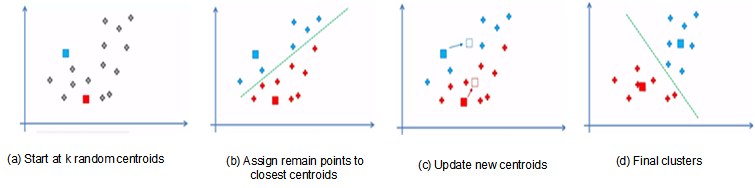
\includegraphics[width=15cm]{kmeans-mechanism}
    \caption{k-means clustering algorithm}\label{fig:kmeans}
\end{figure}  

Due to its simplicity, fast computation, and ability to deal with various data types, k-means is selected as a baseline in this research. 

\subsubsection{Genie}

The second clustering method selected for this research is Genie, a fast hierarchical-based clustering method, recently proposed by \cite{gagolewskiGenieNewFast2016a}. Hierarchy clustering allows to divide a cluster into subgroups, or "nested" clusters, which construct a hierarchy tree of clusters. It is different with a "flatten" clustering like partitioning methods. Besides, Genie’s performance is proved to be unaffected by outliers.

A normal hierarchy cluster tree can be built from bottom up, which means each data point from the beginning is considered as a single cluster, and the pair of data points from two clusters with minimum distance will be merged into one larger cluster. The iteration of merging continues with other pairs of the remain clusters until no pair left unmerged. That indicates the finish of the bottom layer of the tree. The second and higher layers are also constructed by the same criterion: clusters that have the closest pair of data points will be merged. When the top layer only has one large cluster, the tree is completely built. 

However, a Genie cluster tree has one difference in merging criterion to ensure the sizes are not so unequal between clusters, which leads to its advantage of being less sensitive to outliers. The merging criterion is based on a threshold of an economic inequity measure (the Gini index, for instance): smaller clusters are forced to merge if the Gini index of those cluster sizes is higher than the threshold. Thus, the Gini index is updated after each operation of merging (see Equation \eqref{eq:gini_index} for incremental computation of Gini index). That is also the reason why Genie is considered a fast computation method, with $O(n)$ operations rather than $O(n^{2})$ like other traditional hierarchical clustering methods.

At the beginning, every cluster has the same size of 1, thus, the Gini index is 0. If denoting $g_{j}$ as the Gini index value at the time when there are $n − j$ clusters, $j = 0, 1, ..., n − 1$, $g_{j}$ will be computed as in Equation \eqref{eq:gini_index}, where $c_{s_{1}}$ and $c_{s_{2}}$ are the cluster sizes obtained when operating clustering from step $j-1$ to $j$.

\begin{equation}\label{eq:gini_index}
    g_{j} = \dfrac{(n-j)ng_{j-1} + \sum_{i=1}^{n-j+1} (|c_{i} - c_{s_{1}} - c_{s_{2}}| - |c_{i} - c_{s_{1}}| - |c_{i} - c_{s_{2}}|) - c_{s_{2}} - c_{s_{1}} + |c_{s_{1}} - c_{s_{2}}|}{(n-j-1)n}
\end{equation}

\subsubsection{HDBSCAN}

\gls{hdbscan}, introduced by \cite{campelloDensitybasedClusteringBased2013}, is a density-based clustering algorithm, which means the clustering is operated based on the density of the data points: the denser the area is, the higher ability a cluster is formed. However, unlike Genie and k-means, which are complete clustering methods with all points belonging to one cluster, \gls{hdbscan} will ignore sparse regions and marked them as noises during the process of clustering. This is also the reason why \gls{hdbscan} is called the outlier detector. 

Next, one may ask how \gls{hdbscan} can estimate the density of the points to make decision of forming clusters or marking noises. This estimation will be done indirectly through the user pre-set minimum samples hyperparameter. For example, the minimum samples is set as 7, \gls{hdbscan} will compute the furthest distance a point has to travel to reach its closest 7 points. That distance is called core distance, and density is estimated by taking the inverse of core distance. As easily realized in Figure \ref{fig:hdbscan_core_distance}, smaller core distances indicate denser areas and vice versa, sparser regions contains points with larger core distances.

\begin{figure}[h!]
    \centering
    \captionsetup{justification=centering}
    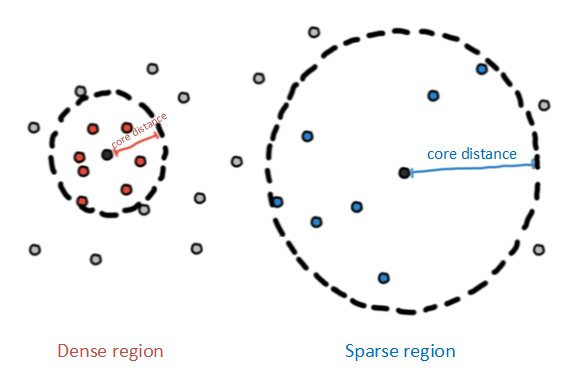
\includegraphics[width=14cm]{hdbscan_core_distance}
    \caption{\gls{hdbscan} core distance}\label{fig:hdbscan_core_distance}
\end{figure}  

After computing the core distances of all points, the mutual reachability distances between each pair of points need to be obtained using Equation \eqref{eq:mrd}

\begin{equation}\label{eq:mrd}
    d_{mreach-k}(a-b) = max\{core_{k}(a),core_{k}(b),d(a,b)\}
\end{equation}

where $core_{k}(a)$ and $core_{k}(b)$ are the core distance for $k$ min samples of point $a$ and point $b$, respectively; $d(a,b)$ is the original distance between point $a$ and point $b$. 

Unlike Genie method, an \gls{hdbscan} cluster tree is formed from top to bottom, which means the splitting will begin from a single large cluster. Next, with a threshold value ($\lambda$), if any mutual reachability distance is higher than the threshold, which means the points are not close enough and not in the dense region, the tree is splitted into smaller clusters. Gradually decrease the threshold value, the splitting operation continue until the threshold cannot be lower. Finally, a complete cluster tree based on density levels is constructed.

\begin{figure}[h!]
    \centering
    \captionsetup{justification=centering}
    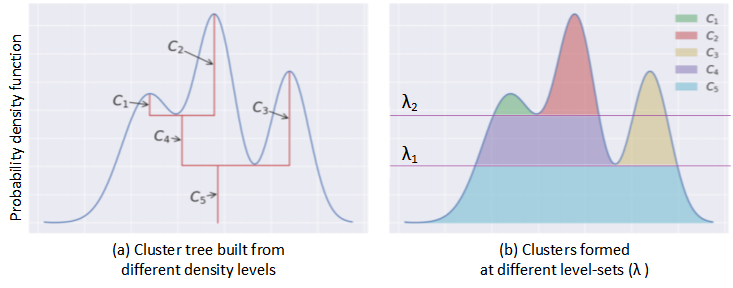
\includegraphics[width=14cm]{hdbscan_density_cluster_tree}
    \caption{\gls{hdbscan} clusters formed based on different density levels}\label{fig:hdbscan_density_cluster_tree}
\end{figure}  

Moreover, \gls{hdbscan} allows users to decide which clusters are important enough to keep based on the hyperparameter minimum cluster size. If during the process of splitting the clusster tree, any cluster smaller than the minimum cluster size will be dropped out of the final cluster tree. This will help smoothing the density probability to reach the real cluster (see Figure \ref{fig:hdbscan_trimmed_density}).

\begin{figure}[h!]
    \centering
    \captionsetup{justification=centering}
    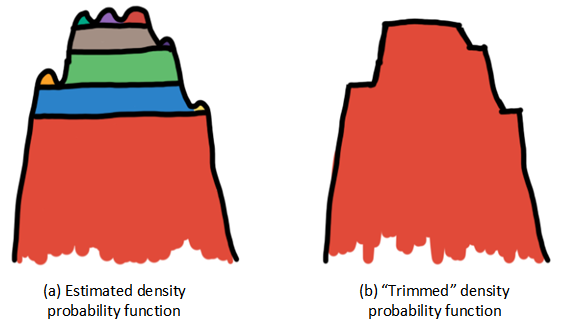
\includegraphics[width=14cm]{hdbscan_trimmed_density}
    \caption{\gls{hdbscan} density probability after filtering small clusters}\label{fig:hdbscan_trimmed_density}
\end{figure}  

Instead of pre-defining number of clusters like k-means, \gls{hdbscan} will return the number of clusters automatically from the internal working mechanism. The only hyper parameters needed to feed into \gls{hdbscan} model are the minimum samples and the minimum cluster size. Besides, it is fast, which makes it suitable to deal with large dataset, such as this thesis project.

\subsubsection{LDA}

\gls{lda} is a statistical modelling method proposed by \cite{blei2003latent}. 
\gls{lda} is selected for this research because it can handle text data directly, without the need to use numerical representation such as text embeddings like other methods discussed above (k-means, Genie, and \gls{hdbscan}). 

\gls{lda} belongs to probability-based clustering method because it works based on assumption of probability distribution: each document is a distribution over topics, and
each topic is a distribution over words. In other words, one document can be assigned more than one topic, and in one topic, some words may show up more than other words. The number of topics $N$ is pre-defined by user.

\begin{figure}[h!]
    \centering
    \captionsetup{justification=centering}
    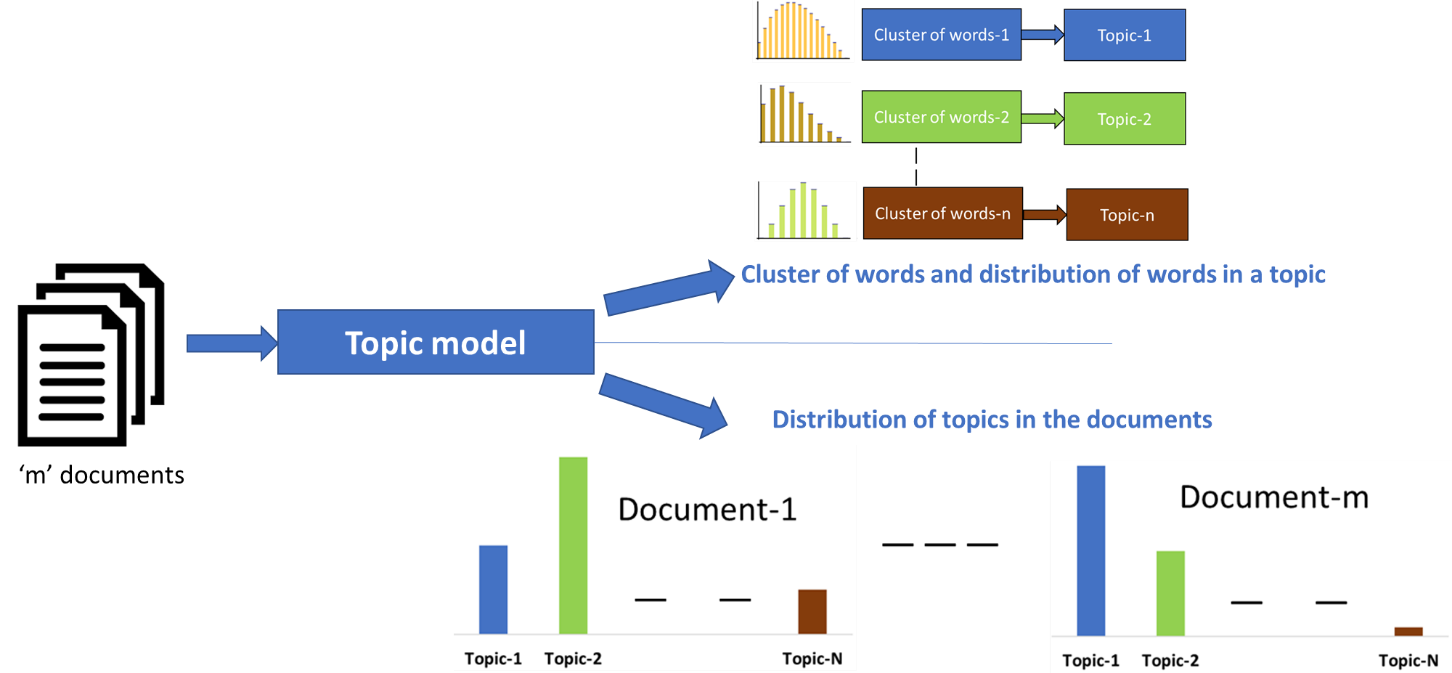
\includegraphics[width=14cm]{lda_distribution}
    \caption{\gls{lda} topic modelling}\label{fig:lda_distribution}
\end{figure}  

Next, to generate the multinomial probabilities of topics for each document and of words per topic, assuming those probabilities have Dirichlet prior distributions, \gls{lda} needs the user to set two Dirichlet priors: alpha and beta. Alpha controls the density of topics per document, which means higher alpha leads to more topics assigned to each document while lower alpha means a document consist only few topic. Meanwhile, beta determines the distribution of words per topic, lower beta means few words per topic and vice versa, higher beta leads to many words contained in each topic. Generally, it is expected that each document should have not many topics assigned and only a few words representing each topic. Thus, alpha and beta should be set at values less than 1. 

\subsubsection{GSDMM}

\gls{gsdmm} is short for the Dirichlet Multinomial Mixture model using collapsed Gibbs Sampling algorithm, proposed by \cite{yinDirichletMultinomialMixture2014}. Similar to \gls{lda}, \gls{gsdmm} is also based on probability of topic distribution per document and word distribution per topic. However, each document can only consist one topic, which makes it suitable for short text clustering. This is also the reason that \gls{gsdmm} is selected for this thesis project. Besides, there is no need to pre-set the number of topics, because the algorithm will do that task by itself. Instead, the maximum number of possible topics, $K$, need to be pre-defined by user. The authors advised that $K$ should be set higher than the expected number of topics, because the final assigned topics may be less than $K$.

\gls{gsdmm} process starts with randomly assigning the documents to $K$ topics. Afterward, the documents are reassigned to the other topics, following two rules:

\begin{itemize}
    \item Rule 1: The document will be reassigned to the topic with more documents.
    \item Rule 2: The documents belonging to the reassigned topic contain more same words with the current document.
\end{itemize}

The loop continues until it reaches the max iterations. Finally, one can observe that some topics consist several documents and some topics are empty, and the documents of the same topic contain similar words. Similar to \gls{lda}, \gls{gsdmm} also needs to pre-define alpha and beta. In the case of \gls{gsdmm}, alpha influences Rule 1 and beta impacts Rule 2. The authors of \gls{gsdmm} used an analogy to describe that process, namely the Movie Group Process, where topics are tables, documents are students, and words are the movies. 

\section{Experiment Setup}



\section{Results}



\section{Discussion}



\section{Conclusion}



\section{Acknowledgements}



\bibliography{Cited}

\end{document}
